\section{Evaluation}
\FloatBarrier

\subsection{400 samples, local max pooling}
\todo[inline]{Turn this into actual text}
T-test probability that the AoC distributions are the same: 0.009790328758564197
T-test probability that the F1 distributions are the same: 0.011943604700946929
\begin{table}[htb]
  \centering
  \begin{tabular}{lrrrr}
    \toprule
    model & \multicolumn{2}{c}{F1} & \multicolumn{2}{c}{AoC} \\
    \cmidrule(l){2-3} \cmidrule(l){4-5}
    & mean & std & mean & std \\
    \midrule
    CNN & 0.79126 & 0.01644 & 0.856768 & 0.0219711 \\
    CNN-clusters & 0.83429 & 0.02047 & 0.904359 & 0.0168642 \\
    \bottomrule
  \end{tabular}
  \caption{Performance metrics on a small dataset (200 positive
    samples)}
  \label{tbl:small}
\end{table}

\begin{figure}[htb]
  \centering
  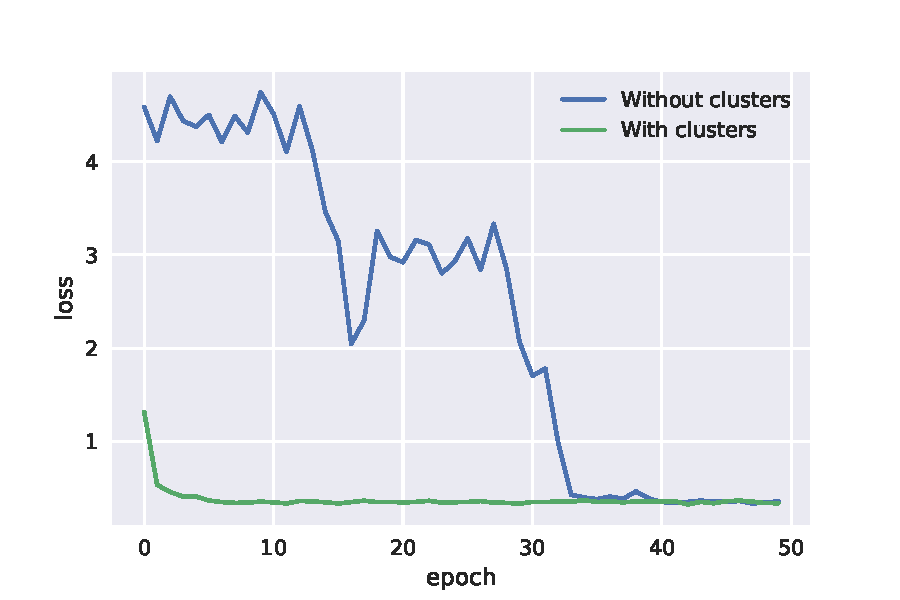
\includegraphics[width=\textwidth]{figures/results/small_5_fold_convergence.pdf}
  \caption{The convergence speed}
  \label{fig:small_convergence}
\end{figure}

\begin{figure}[htb]
  \centering
  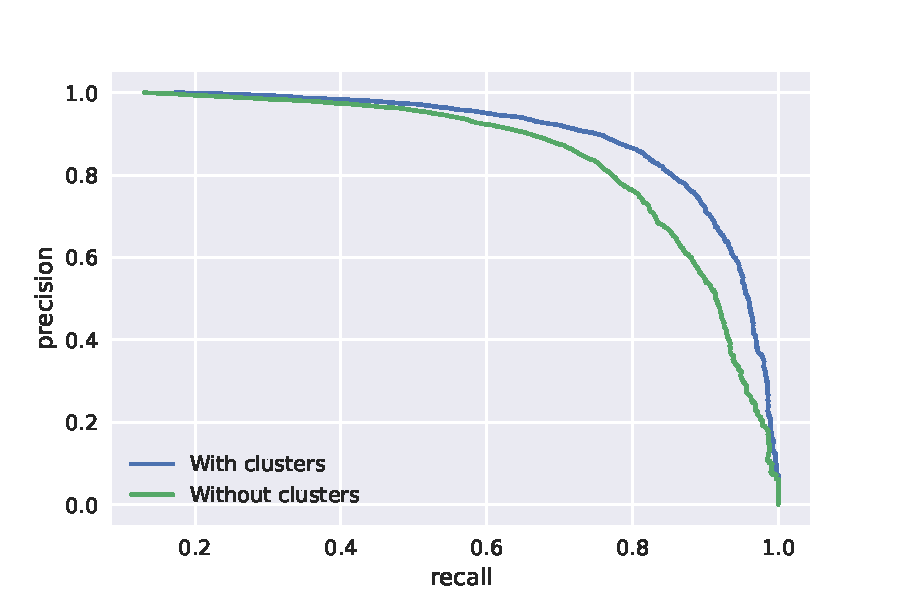
\includegraphics[width=\textwidth]{figures/results/small_5_fold_pr.pdf}
  \caption{The precision/recall curves}
  \label{fig:small_convergence}
\end{figure}

\begin{figure}[htb]
  \centering
  \begin{subfigure}[b]{0.80\textwidth} 
    \centering
    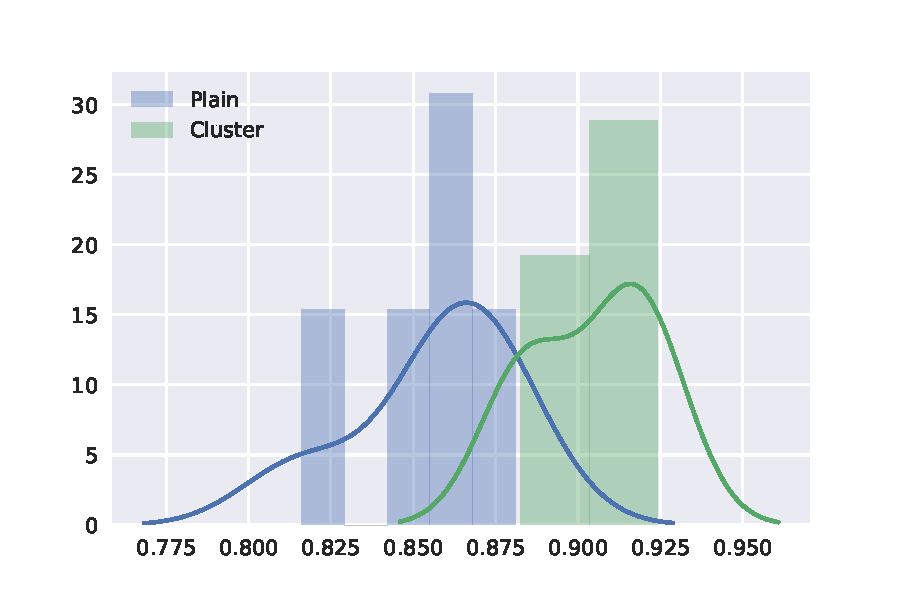
\includegraphics[width=\textwidth]{figures/results/small_5_fold_kde.pdf}
    \caption{Kernel density estimation}
  \end{subfigure}
  \vspace{0.10\textwidth}
  \begin{subfigure}[b]{0.80\textwidth}
	\centering
    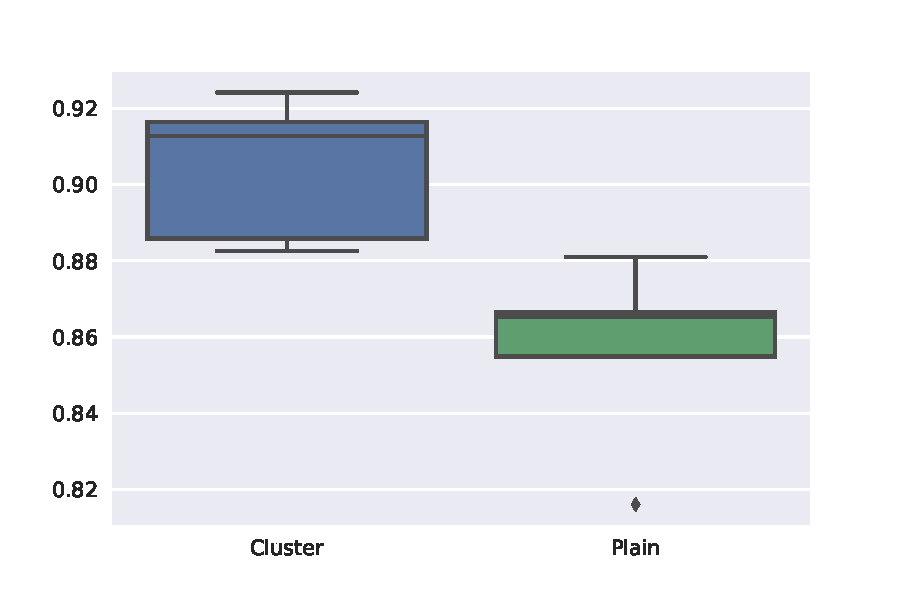
\includegraphics[width=\textwidth]{figures/results/small_5_fold_boxplot.pdf}
    \caption{Boxplot}
  \end{subfigure}
  \caption{The distribution of the cross validation results}
  \label{fig:small_dist}
\end{figure}

\subsection{400 samples, 1-max pooling}
\begin{figure}[htb]
  \centering
  \begin{subfigure}[b]{0.49\textwidth} 
    \centering
    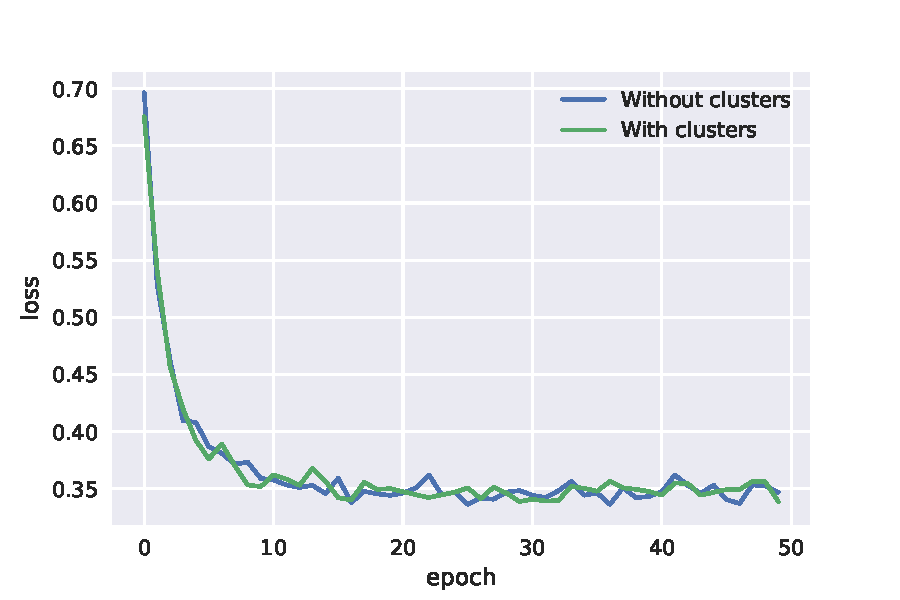
\includegraphics[width=\textwidth]{figures/results/datasize/200pos_10fold_default_losses.pdf}
    \caption{Average loss at each epoch}
  \end{subfigure}
  \begin{subfigure}[b]{0.49\textwidth}
	\centering
    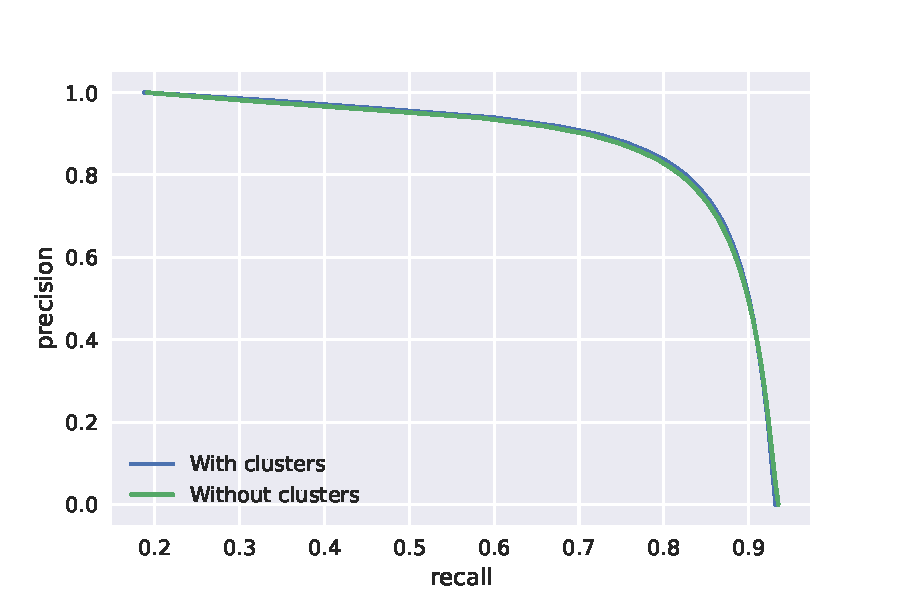
\includegraphics[width=\textwidth]{figures/results/datasize/200pos_10fold_default_pr.pdf}
    \caption{Average precision/recall curve}
  \end{subfigure}
  \begin{subfigure}[b]{0.49\textwidth}
	\centering
    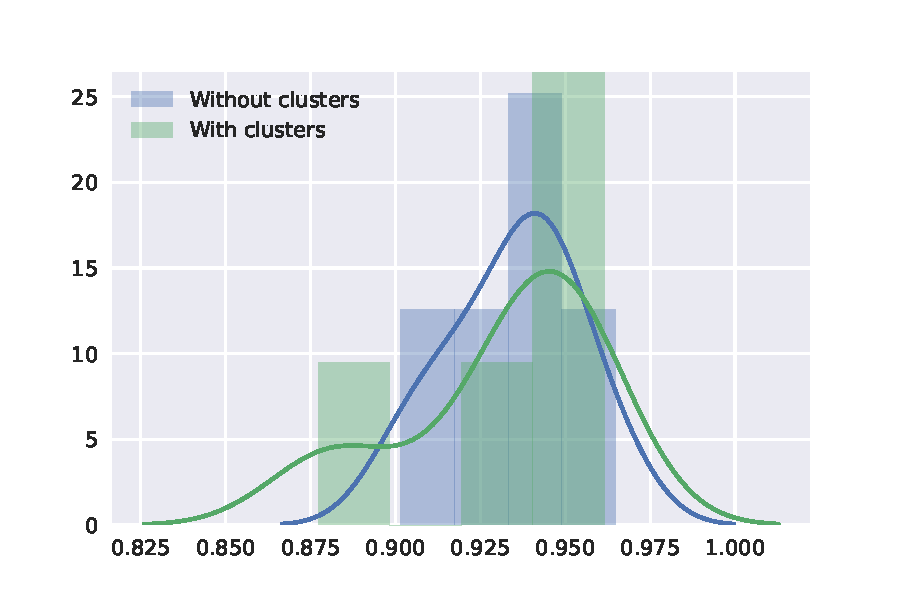
\includegraphics[width=\textwidth]{figures/results/datasize/200pos_10fold_default_kde_ap.pdf}
    \caption{Kernel density estimation of average precision}
  \end{subfigure}
  \begin{subfigure}[b]{0.49\textwidth}
	\centering
    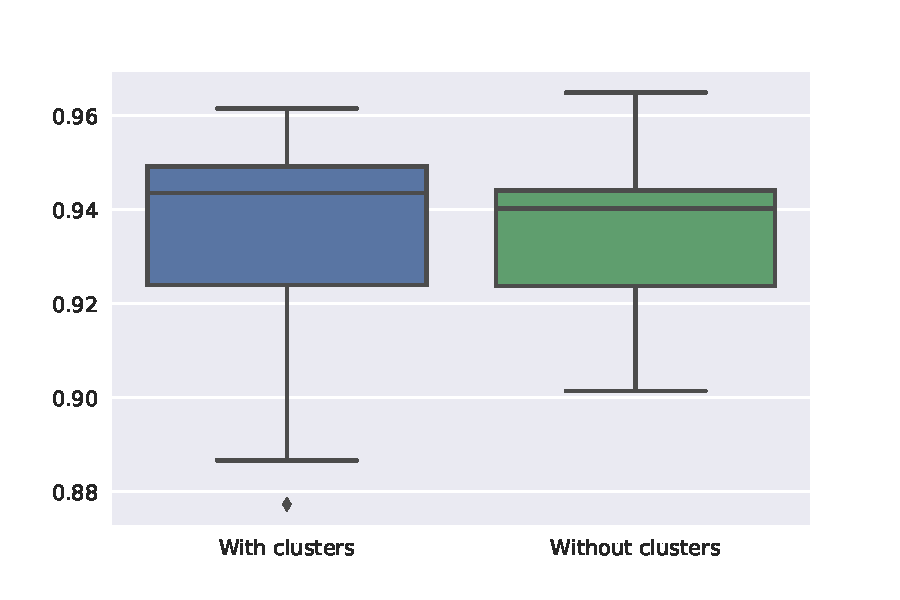
\includegraphics[width=\textwidth]{figures/results/datasize/200pos_10fold_default_boxplot_ap.pdf}
    \caption{Box plot of average precision}
  \end{subfigure}
  \begin{subfigure}[b]{0.49\textwidth}
	\centering
    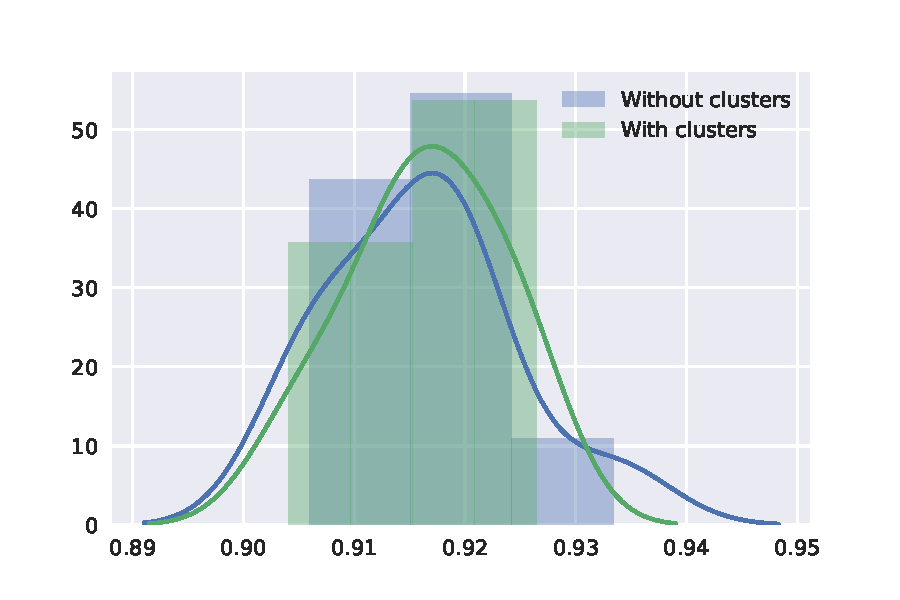
\includegraphics[width=\textwidth]{figures/results/datasize/200pos_10fold_default_kde_f1.pdf}
    \caption{Kernel density estimation of F1 score}
  \end{subfigure}
  \begin{subfigure}[b]{0.49\textwidth}
	\centering
    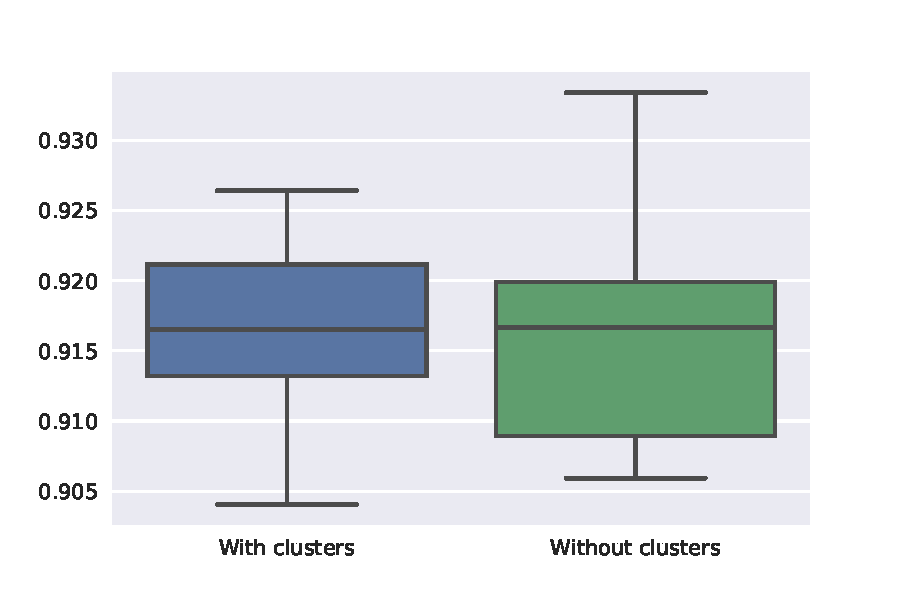
\includegraphics[width=\textwidth]{figures/results/datasize/200pos_10fold_default_boxplot_f1.pdf}
    \caption{Box plot of F1 score}
  \end{subfigure}
  \caption{At 200 positive and 200 negative samples with 1-max pooling, there is
    no discernable difference between the two models.}
  \label{fig:200_1max}
\end{figure}

\begin{table}[htb]
  \centering
  \begin{tabular}{lrrrr}
    \toprule
    model & \multicolumn{2}{c}{F1} & \multicolumn{2}{c}{AoC} \\
    \cmidrule(l){2-3} \cmidrule(l){4-5}
    & mean & std & mean & std \\
    \midrule
    CNN & 0.916071 & 0.00786046 & 0.934946 & 0.0183115 \\
    CNN-clusters & 0.916407 & 0.00664848 & 0.931635 & 0.0270519 \\
    \bottomrule
  \end{tabular}
  \caption{Performance metrics on 200 positive and 200 negative samples with
    1-max pooling. The T-test probability of the null hypothesis being true for
    the average precision is 0.765, for the F1 score it is 0.923. This makes it
    fairly save to say that for this configuration there is no benefit to the
    addition of clustering data.
    }
  \label{tbl:200pos_1max}
\end{table}

\FloatBarrier

%%% Local Variables:
%%% mode: latex
%%% TeX-master: "report"
%%% End: